\documentclass{beamer}


\usepackage[utf8]{inputenc}
\usepackage{pgfpages}
\usepackage{xcolor}

\setbeameroption{show notes}
\setbeamertemplate{note page}[plain]
\setbeameroption{show notes on second screen=left}

\usetheme{Warsaw}
\graphicspath{ {./images/}{../images/}{../kcov-swedencpp/images/}{../../kcov-swedencpp/images/} }

\AtBeginSection[specialframe]
{
  \begin{frame}{Table of Contents}
   \tableofcontents[currentsection]
  \end{frame}
}

\title[Kcov - a single-step code coverage tool] %optional
{Kcov - a single-step code coverage tool}

%\subtitle{A short story}

\author{Simon Kågström}

\institute
{
  Consultant\\
  \texttt{https://github.com/SimonKagstrom/emilpro}
}

%\logo{\includegraphics[height=1.5cm]{lion-logo.png}}

\begin{document}

\begin{frame}
  \titlepage
  \note{My name is Simon Kågström and I work as a consultant, currently at Profoto. Tonight I will present emilpro.

So let's get started!}
\end{frame}

\begin{frame}
  \frametitle{Motivation}
  \note<1->{
    \footnotesize
  }

  \note<2>{

  %\includegraphics<1>[height=8cm]{goto_fail_no_coverage}
  %\includegraphics<2>[height=8cm]{goto_fail}
\end{frame}


\begin{frame}{Actors and objects}
    % Sections, symbols, relocations
    % Disassembler, compiler, linker, loader
    \end{frame}

\begin{frame}{Why is this easier now than 10 years ago?}
    %conan
    %copilot
    %move from binutils
\end{frame}

\begin{frame}{Questions and comments!}
  \footnotesize
  (Images from \url{http://www.falselogic.net/LetsPlay/SpaceQuest.html})
  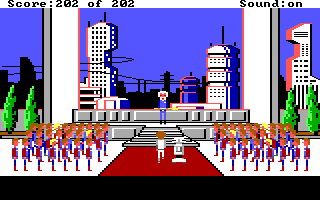
\includegraphics[width=\linewidth]{sq_final}
\end{frame}

\end{document}
